\begin{tabular}[ht]{M{2.cm}M{2.cm}M{4.cm}M{4.cm}N}
  %\setlength\extrarowheight{2.5pt}
  \hline
  \multicolumn{2}{c}{Particles in cells} & \multicolumn{2}{c}{Critical Courant number $a\Delta t /\Delta X = f(a/b)$}  & \\[0.5cm]
  & &  DCU & CTU & \\
%   & & \multicolumn{2}{c}{$a/b=1$} & \multicolumn{2}{c}{$a/b=10$} & \multicolumn{2}{c}{$a/b=1$} & \multicolumn{2}{c}{$a/b=10$}\\
   % Particles & Position of particles in cell $c$ &  \multicolumn{2}{c}{DCU} & \multicolumn{2}{c}{DCU} \\
  \hline
  \hline
  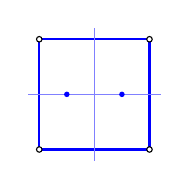
\begin{tikzpicture}[scale=0.7]
    \draw[Blue,thick] (-1.,-1.) rectangle (1.,1.);
    \draw[Blue!50] (-1.2,0.) -- (1.2,0.0);\draw[Blue!50] (.0,-1.2) -- (0.,1.2);
    %% nodes
    \fill[white] (-1,-1) circle (0.05);\draw (-1,-1) circle (0.05);
    \fill[white] (1.,-1) circle (0.05);\draw (1,-1) circle (0.05);
    \fill[white] (1,1) circle (0.05);\draw (1,1) circle (0.05);
    \fill[white] (-1.,1) circle (0.05);\draw (-1,1) circle (0.05);
    %% particles
    \fill[Blue] (-0.5,0.) circle (0.05);
    \fill[Blue] (0.5,0.) circle (0.05);
  \end{tikzpicture} & 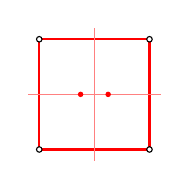
\begin{tikzpicture}[scale=0.7]
    \draw[Red,thick] (-1.,-1.) rectangle (1.,1.);
    \draw[Red!50] (-1.2,0.) -- (1.2,0.0);\draw[Red!50] (.0,-1.2) -- (0.,1.2);
    %% nodes
    \fill[white] (-1,-1) circle (0.05);\draw (-1,-1) circle (0.05);
    \fill[white] (1.,-1) circle (0.05);\draw (1,-1) circle (0.05);
    \fill[white] (1,1) circle (0.05);\draw (1,1) circle (0.05);
    \fill[white] (-1.,1) circle (0.05);\draw (-1,1) circle (0.05);
    %% particles
    \fill[Red] (-0.25,0.) circle (0.05);
    \fill[Red] (0.25,0.) circle (0.05);
  \end{tikzpicture}  & 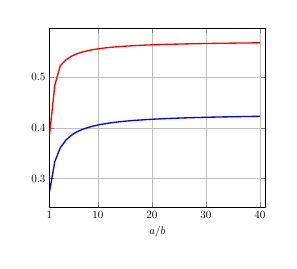
\begin{tikzpicture}[scale=0.4]
\begin{axis}[xlabel=$a/b$,ymajorgrids=true,xmajorgrids=true,xmin=1,xmax=41,xtick={1,10,20,30,40}]
%%%%%%%%%%% NATURAL CONFIGURATION
\addplot[Blue,very thick] coordinates {(1.0,0.272727272727) (2.0,0.333333333333) (3.0,0.36) (4.0,0.375) (5.0,0.384615384615) (6.0,0.391304347826) (7.0,0.396226415094) (8.0,0.4) (9.0,0.402985074627) (10.0,0.405405405405) (11.0,0.407407407407) (12.0,0.409090909091) (13.0,0.410526315789) (14.0,0.411764705882) (15.0,0.412844036697) (16.0,0.413793103448) (17.0,0.414634146341) (18.0,0.415384615385) (19.0,0.416058394161) (20.0,0.416666666667) (21.0,0.417218543046) (22.0,0.417721518987) (23.0,0.418181818182) (24.0,0.418604651163) (25.0,0.418994413408) (26.0,0.41935483871) (27.0,0.419689119171) (28.0,0.42) (29.0,0.420289855072) (30.0,0.420560747664) (31.0,0.420814479638) (32.0,0.421052631579) (33.0,0.421276595745) (34.0,0.421487603306) (35.0,0.421686746988) (36.0,0.421875) (37.0,0.422053231939) (38.0,0.422222222222) (39.0,0.42238267148) (40.0,0.422535211268) };
%%%%%%%%%%% MODIFIED CONFIGURATION
\addplot[Red,very thick] coordinates {(1.0,0.384615384615) (2.0,0.483870967742) (3.0,0.521739130435) (4.0,0.533333333333) (5.0,0.540540540541) (6.0,0.545454545455) (7.0,0.549019607843) (8.0,0.551724137931) (9.0,0.553846153846) (10.0,0.555555555556) (11.0,0.556962025316) (12.0,0.558139534884) (13.0,0.559139784946) (14.0,0.56) (15.0,0.560747663551) (16.0,0.561403508772) (17.0,0.561983471074) (18.0,0.5625) (19.0,0.562962962963) (20.0,0.56338028169) (21.0,0.563758389262) (22.0,0.564102564103) (23.0,0.564417177914) (24.0,0.564705882353) (25.0,0.564971751412) (26.0,0.565217391304) (27.0,0.565445026178) (28.0,0.565656565657) (29.0,0.565853658537) (30.0,0.566037735849) (31.0,0.566210045662) (32.0,0.566371681416) (33.0,0.56652360515) (34.0,0.566666666667) (35.0,0.566801619433) (36.0,0.566929133858) (37.0,0.567049808429) (38.0,0.567164179104) (39.0,0.567272727273) (40.0,0.567375886525) };
\end{axis}
\end{tikzpicture}
%%% Local Variables:
%%% mode: latex
%%% TeX-master: "../../mainManuscript"
%%% End:
 & 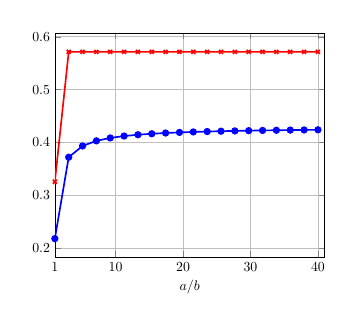
\begin{tikzpicture}[scale=0.5]
\begin{axis}[xlabel=$a/b$,ymajorgrids=true,xmajorgrids=true,xmin=1,xmax=41,xtick={1,10,20,30,40}]
%%%%%%%%%%% NATURAL CONFIGURATION
\addplot[Blue,mark=*,very thick] coordinates {(1.0,0.217751156849) (3.05263157895,0.371899923259) (5.10526315789,0.393212462993) (7.15789473684,0.402887246166) (9.21052631579,0.40840759179) (11.2631578947,0.411975544) (13.3157894737,0.414470966386) (15.3684210526,0.416314181564) (17.4210526316,0.417731290591) (19.4736842105,0.418854723411) (21.5263157895,0.419767189778) (23.5789473684,0.420523008979) (25.6315789474,0.421159327636) (27.6842105263,0.421702408465) (29.7368421053,0.422171344199) (31.7894736842,0.422580347983) (33.8421052632,0.422940218545) (35.8947368421,0.423259307375) (37.9473684211,0.423544174777) (40.0,0.423800045624) };
%%%%%%%%%%% MODIFIED CONFIGURATION
\addplot[Red,mark=x,very thick] coordinates {(1.0,0.325412497399) (3.05263157895,0.571428571428) (5.10526315789,0.571428571429) (7.15789473684,0.571428571429) (9.21052631579,0.57142857143) (11.2631578947,0.571428571429) (13.3157894737,0.571428571429) (15.3684210526,0.571428571429) (17.4210526316,0.571428571429) (19.4736842105,0.571428571429) (21.5263157895,0.571428571429) (23.5789473684,0.571428571429) (25.6315789474,0.571428571429) (27.6842105263,0.571428571429) (29.7368421053,0.571428571429) (31.7894736842,0.571428571429) (33.8421052632,0.571428571429) (35.8947368421,0.571428571429) (37.9473684211,0.571428571429) (40.0,0.571428571429) };
\end{axis}
\end{tikzpicture}
%%% Local Variables:
%%% mode: latex
%%% TeX-master: "../../mainManuscript"
%%% End:
&\\ [2.75cm]%%% SOLUTION
  \hline
  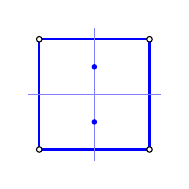
\begin{tikzpicture}[scale=0.7]
    \draw[Blue,thick] (-1.,-1.) rectangle (1.,1.);
    \draw[Blue!50] (-1.2,0.) -- (1.2,0.0);\draw[Blue!50] (.0,-1.2) -- (0.,1.2);
    %% nodes
    \fill[white] (-1,-1) circle (0.05);\draw (-1,-1) circle (0.05);
    \fill[white] (1.,-1) circle (0.05);\draw (1,-1) circle (0.05);
    \fill[white] (1,1) circle (0.05);\draw (1,1) circle (0.05);
    \fill[white] (-1.,1) circle (0.05);\draw (-1,1) circle (0.05);
    %% particles
    \fill[Blue] (0.,-0.5) circle (0.05);
    \fill[Blue] (0.,0.5) circle (0.05);
  \end{tikzpicture} & 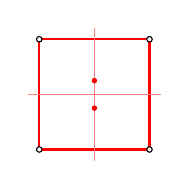
\begin{tikzpicture}[scale=0.7]
    \draw[Red,thick] (-1.,-1.) rectangle (1.,1.);
    \draw[Red!50] (-1.2,0.) -- (1.2,0.0);\draw[Red!50] (.0,-1.2) -- (0.,1.2);
    %% nodes
    \fill[white] (-1,-1) circle (0.05);\draw (-1,-1) circle (0.05);
    \fill[white] (1.,-1) circle (0.05);\draw (1,-1) circle (0.05);
    \fill[white] (1,1) circle (0.05);\draw (1,1) circle (0.05);
    \fill[white] (-1.,1) circle (0.05);\draw (-1,1) circle (0.05);
    %% particles
    \fill[Red] (0.,-0.25) circle (0.05);
    \fill[Red] (0.,0.25) circle (0.05);
  \end{tikzpicture} & 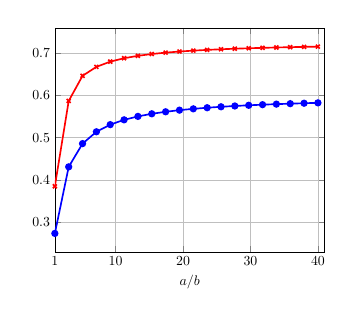
\begin{tikzpicture}[scale=0.5]
\begin{axis}[xlabel=$a/b$,ymajorgrids=true,xmajorgrids=true,xmin=1,xmax=41,xtick={1,10,20,30,40}]
%%%%%%%%%%% NATURAL CONFIGURATION
\addplot[Blue,mark=*,very thick] coordinates {(1.0,0.272727272727) (3.05263157895,0.430693069307) (5.10526315789,0.485809682805) (7.15789473684,0.513853904282) (9.21052631579,0.530839231547) (11.2631578947,0.54222972973) (13.3157894737,0.550398839739) (15.3684210526,0.556543837357) (17.4210526316,0.561334087055) (19.4736842105,0.56517311609) (21.5263157895,0.568318666049) (23.5789473684,0.570943075616) (25.6315789474,0.57316594743) (27.6842105263,0.575072886297) (29.7368421053,0.576726777816) (31.7894736842,0.578174856414) (33.8421052632,0.579453289276) (35.8947368421,0.580590238365) (37.9473684211,0.581607959129) (40.0,0.582524271845) };
%%%%%%%%%%% MODIFIED CONFIGURATION
\addplot[Red,mark=x,very thick] coordinates {(1.0,0.384615384615) (3.05263157895,0.587044534413) (5.10526315789,0.646666666667) (7.15789473684,0.667894413751) (9.21052631579,0.680272108844) (11.2631578947,0.688379573784) (13.3157894737,0.694101508916) (15.3684210526,0.698355754858) (17.4210526316,0.70164281929) (19.4736842105,0.704258862717) (21.5263157895,0.706390328152) (23.5789473684,0.7081604426) (25.6315789474,0.709653916211) (27.6842105263,0.71093090049) (29.7368421053,0.712035286704) (31.7894736842,0.712999852442) (33.8421052632,0.713849569803) (35.8947368421,0.714603798297) (37.9473684211,0.715277777778) (40.0,0.715883668904) };
\end{axis}
\end{tikzpicture}
%%% Local Variables:
%%% mode: latex
%%% TeX-master: "../../mainManuscript"
%%% End:
 & 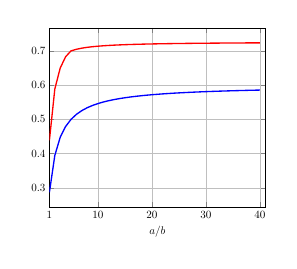
\begin{tikzpicture}[scale=0.4]
\begin{axis}[xlabel=$a/b$,ymajorgrids=true,xmajorgrids=true,xmin=1,xmax=41,xtick={1,10,20,30,40}]
%%%%%%%%%%% NATURAL CONFIGURATION
\addplot[Blue,very thick] coordinates {(1.0,0.286705918022) (2.0,0.394448724536) (3.0,0.447656821925) (4.0,0.479202710604) (5.0,0.5) (6.0,0.514718625761) (7.0,0.525674830612) (8.0,0.534143900269) (9.0,0.540884552925) (10.0,0.546375952926) (11.0,0.550935403911) (12.0,0.554781280898) (13.0,0.558068753046) (14.0,0.560911085414) (15.0,0.56339287739) (16.0,0.565578584542) (17.0,0.567518173117) (18.0,0.56925097228) (19.0,0.570808360078) (20.0,0.572215675072) (21.0,0.57349360201) (22.0,0.574659192897) (23.0,0.575726630632) (24.0,0.576707807868) (25.0,0.577612771199) (26.0,0.578450065864) (27.0,0.579227006022) (28.0,0.579949888678) (29.0,0.58062416451) (30.0,0.581254575404) (31.0,0.581845266009) (32.0,0.582399874872) (33.0,0.58292160939) (34.0,0.583413307817) (35.0,0.583877490879) (36.0,0.58431640496) (37.0,0.584732058433) (38.0,0.585126252361) (39.0,0.585500606572) (40.0,0.585856581891) };
%%%%%%%%%%% MODIFIED CONFIGURATION
\addplot[Red,very thick] coordinates {(1.0,0.438891399031) (2.0,0.589023983378) (3.0,0.650325753638) (4.0,0.683375209645) (5.0,0.700574756943) (6.0,0.705224542261) (7.0,0.708497377871) (8.0,0.710925299709) (9.0,0.712797780481) (10.0,0.714285714286) (11.0,0.715496454998) (12.0,0.716500819965) (13.0,0.717347407474) (14.0,0.718070673576) (15.0,0.718695725716) (16.0,0.719241290941) (17.0,0.719721621044) (18.0,0.720147753708) (19.0,0.720528370019) (20.0,0.720870391403) (21.0,0.7211794039) (22.0,0.721459965346) (23.0,0.7217158315) (24.0,0.721950125023) (25.0,0.722165463462) (26.0,0.722364057406) (27.0,0.722547786604) (28.0,0.722718259617) (29.0,0.722876861023) (30.0,0.723024789078) (31.0,0.723163086043) (32.0,0.723292662763) (33.0,0.723414318746) (34.0,0.723528758668) (35.0,0.723636606028) (36.0,0.723738414512) (37.0,0.723834677494) (38.0,0.723925836029) (39.0,0.724012285615) (40.0,0.724094381918) };
\end{axis}
\end{tikzpicture}
%%% Local Variables:
%%% mode: latex
%%% TeX-master: "../../mainManuscript"
%%% End:
& \\ [2.75cm] %%% SOLUTION
  \hline
  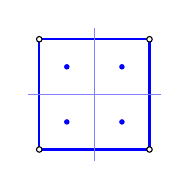
\begin{tikzpicture}[scale=0.7]
    \draw[Blue,thick] (-1.,-1.) rectangle (1.,1.);
    \draw[Blue!50] (-1.2,0.) -- (1.2,0.0);\draw[Blue!50] (.0,-1.2) -- (0.,1.2);
    %% nodes
    \fill[white] (-1,-1) circle (0.05);\draw (-1,-1) circle (0.05);
    \fill[white] (1.,-1) circle (0.05);\draw (1,-1) circle (0.05);
    \fill[white] (1,1) circle (0.05);\draw (1,1) circle (0.05);
    \fill[white] (-1.,1) circle (0.05);\draw (-1,1) circle (0.05);
    %% particles
    \fill[Blue] (-0.5,-0.5) circle (0.05);
    \fill[Blue] (0.5,-0.5) circle (0.05);
    \fill[Blue] (0.5,0.5) circle (0.05);
    \fill[Blue] (-0.5,0.5) circle (0.05);
  \end{tikzpicture} & 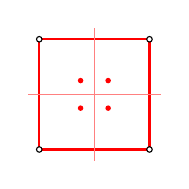
\begin{tikzpicture}[scale=0.7]
    \draw[Red,thick] (-1.,-1.) rectangle (1.,1.);
    \draw[Red!50] (-1.2,0.) -- (1.2,0.0);\draw[Red!50] (.0,-1.2) -- (0.,1.2);
    %% nodes
    \fill[white] (-1,-1) circle (0.05);\draw (-1,-1) circle (0.05);
    \fill[white] (1.,-1) circle (0.05);\draw (1,-1) circle (0.05);
    \fill[white] (1,1) circle (0.05);\draw (1,1) circle (0.05);
    \fill[white] (-1.,1) circle (0.05);\draw (-1,1) circle (0.05);
    %% particles
    \fill[Red] (-0.25,-0.25) circle (0.05);
    \fill[Red] (0.25,-0.25) circle (0.05);
    \fill[Red] (0.25,0.25) circle (0.05);
    \fill[Red] (-0.25,0.25) circle (0.05);
  \end{tikzpicture}&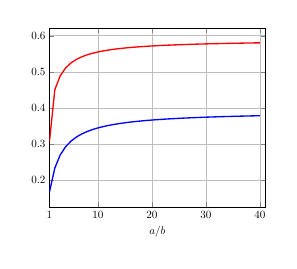
\begin{tikzpicture}[scale=0.4]
\begin{axis}[xlabel=$a/b$,ymajorgrids=true,xmajorgrids=true,xmin=1,xmax=41,xtick={1,10,20,30,40}]
%%%%%%%%%%% NATURAL CONFIGURATION
\addplot[Blue,very thick] coordinates {(1.0,0.166666666667) (2.0,0.233766233766) (3.0,0.27) (4.0,0.292682926829) (5.0,0.308219178082) (6.0,0.319526627219) (7.0,0.328125) (8.0,0.33488372093) (9.0,0.340336134454) (10.0,0.344827586207) (11.0,0.348591549296) (12.0,0.351791530945) (13.0,0.354545454545) (14.0,0.356940509915) (15.0,0.359042553191) (16.0,0.360902255639) (17.0,0.362559241706) (18.0,0.36404494382) (19.0,0.365384615385) (20.0,0.366598778004) (21.0,0.367704280156) (22.0,0.368715083799) (23.0,0.369642857143) (24.0,0.370497427101) (25.0,0.371287128713) (26.0,0.372019077901) (27.0,0.372699386503) (28.0,0.373333333333) (29.0,0.373925501433) (30.0,0.374479889043) (31.0,0.375) (32.0,0.375488917862) (33.0,0.375949367089) (34.0,0.376383763838) (35.0,0.376794258373) (36.0,0.377182770664) (37.0,0.377551020408) (38.0,0.377900552486) (39.0,0.378232758621) (40.0,0.378548895899) };
%%%%%%%%%%% MODIFIED CONFIGURATION
\addplot[Red,very thick] coordinates {(1.0,0.30612244898) (2.0,0.450574712644) (3.0,0.488913525499) (4.0,0.510638297872) (5.0,0.524625267666) (6.0,0.534383520145) (7.0,0.541578947368) (8.0,0.547103977669) (9.0,0.551479783243) (10.0,0.555031149707) (11.0,0.557971014493) (12.0,0.560444797458) (13.0,0.562555195761) (14.0,0.564376799671) (15.0,0.565965092402) (16.0,0.567362199976) (17.0,0.568600682594) (18.0,0.569706103994) (19.0,0.570698814875) (20.0,0.571595217265) (21.0,0.572408677916) (22.0,0.57315019938) (23.0,0.57382892057) (24.0,0.574452495319) (25.0,0.575027382256) (26.0,0.575559069347) (27.0,0.576052249637) (28.0,0.576510960151) (29.0,0.576938692651) (30.0,0.577338482686) (31.0,0.577712981744) (32.0,0.578064516129) (33.0,0.578395135328) (34.0,0.578706652) (35.0,0.579000675219) (36.0,0.579278638279) (37.0,0.579541822056) (38.0,0.579791374747) (39.0,0.580028328612) (40.0,0.58025361425) };
\end{axis}
\end{tikzpicture}
%%% Local Variables:
%%% mode: latex
%%% TeX-master: "../../mainManuscript"
%%% End:
 & 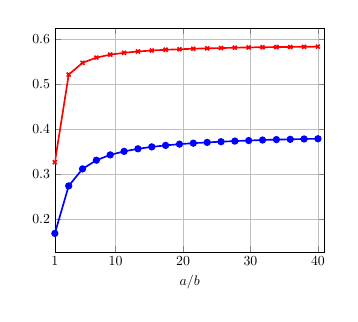
\begin{tikzpicture}[scale=0.5]
\begin{axis}[xlabel=$a/b$,ymajorgrids=true,xmajorgrids=true,xmin=1,xmax=41,xtick={1,10,20,30,40}]
%%%%%%%%%%% NATURAL CONFIGURATION
\addplot[Blue,mark=*,very thick] coordinates {(1.0,0.168781687817) (3.05263157895,0.274434323291) (5.10526315789,0.312241017147) (7.15789473684,0.331556999781) (9.21052631579,0.343371854771) (11.2631578947,0.351188775046) (13.3157894737,0.356866726562) (15.3684210526,0.361161506352) (17.4210526316,0.364452065573) (19.4736842105,0.367277356984) (21.5263157895,0.3693952729) (23.5789473684,0.371136342942) (25.6315789474,0.372686884764) (27.6842105263,0.374017424385) (29.7368421053,0.375282700195) (31.7894736842,0.376391132332) (33.8421052632,0.377343247117) (35.8947368421,0.377975358701) (37.9473684211,0.378718524027) (40.0,0.379203792038) };
%%%%%%%%%%% MODIFIED CONFIGURATION
\addplot[Red,mark=x,very thick] coordinates {(1.0,0.327083270833) (3.05263157895,0.521791533705) (5.10526315789,0.548055480555) (7.15789473684,0.559609806624) (9.21052631579,0.566176714399) (11.2631578947,0.570259386804) (13.3157894737,0.573250469347) (15.3684210526,0.575399438205) (17.4210526316,0.576991033068) (19.4736842105,0.578179466005) (21.5263157895,0.579278950684) (23.5789473684,0.580283697574) (25.6315789474,0.580817387121) (27.6842105263,0.581651079669) (29.7368421053,0.582253190953) (31.7894736842,0.5827068797) (33.8421052632,0.583105304737) (35.8947368421,0.583295306637) (37.9473684211,0.583636362679) (40.0,0.584005840058) };
\end{axis}
\end{tikzpicture}
%%% Local Variables:
%%% mode: latex
%%% TeX-master: "../../mainManuscript"
%%% End:
& \\ [2.75cm]
  %%%%%%%%%%%%%%%%%%%%%%%%%%%%%%%%%%%%%%%
  %%%%%%%%%%%%%%%%%%%%%%%%%%%%%%%%%%%%%%% 
  \hline % Shifted left // Shifted right
  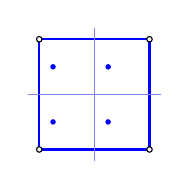
\begin{tikzpicture}[scale=0.7]
    \draw[Blue,thick] (-1.,-1.) rectangle (1.,1.);
    \draw[Blue!50] (-1.2,0.) -- (1.2,0.0);\draw[Blue!50] (.0,-1.2) -- (0.,1.2);
    %% nodes
    \fill[white] (-1,-1) circle (0.05);\draw (-1,-1) circle (0.05);
    \fill[white] (1.,-1) circle (0.05);\draw (1,-1) circle (0.05);
    \fill[white] (1,1) circle (0.05);\draw (1,1) circle (0.05);
    \fill[white] (-1.,1) circle (0.05);\draw (-1,1) circle (0.05);
    %% particles
    \fill[Blue] (-0.5-0.25,-0.5) circle (0.05);
    \fill[Blue] (0.5-0.25,-0.5) circle (0.05);
    \fill[Blue] (0.5-0.25,0.5) circle (0.05);
    \fill[Blue] (-0.5-0.25,0.5) circle (0.05);
  \end{tikzpicture} & 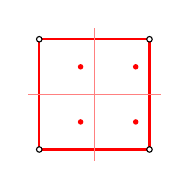
\begin{tikzpicture}[scale=0.7]
    \draw[Red,thick] (-1.,-1.) rectangle (1.,1.);
    \draw[Red!50] (-1.2,0.) -- (1.2,0.0);\draw[Red!50] (.0,-1.2) -- (0.,1.2);
    %% nodes
    \fill[white] (-1,-1) circle (0.05);\draw (-1,-1) circle (0.05);
    \fill[white] (1.,-1) circle (0.05);\draw (1,-1) circle (0.05);
    \fill[white] (1,1) circle (0.05);\draw (1,1) circle (0.05);
    \fill[white] (-1.,1) circle (0.05);\draw (-1,1) circle (0.05);
    %% particles
    \fill[Red] (-0.5+0.25,-0.5) circle (0.05);
    \fill[Red] (0.5+0.25,-0.5) circle (0.05);
    \fill[Red] (0.5+0.25,0.5) circle (0.05);
    \fill[Red] (-0.5+0.25,0.5) circle (0.05);
  \end{tikzpicture} & 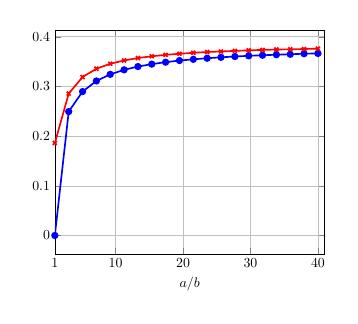
\begin{tikzpicture}[scale=0.5]
\begin{axis}[xlabel=$a/b$,ymajorgrids=true,xmajorgrids=true,xmin=1,xmax=41,xtick={1,10,20,30,40}]
%%%%%%%%%%% NATURAL CONFIGURATION
\addplot[Blue,mark=*,very thick] coordinates {(1.0,1.0000100001e-05) (3.05263157895,0.249310914162) (5.10526315789,0.28957342205) (7.15789473684,0.311013636452) (9.21052631579,0.324305874638) (11.2631578947,0.333392807612) (13.3157894737,0.339955504818) (15.3684210526,0.344870817129) (17.4210526316,0.348772961414) (19.4736842105,0.352087731404) (21.5263157895,0.354541966472) (23.5789473684,0.356753041215) (25.6315789474,0.358589375367) (27.6842105263,0.360175180699) (29.7368421053,0.361603616036) (31.7894736842,0.362721521952) (33.8421052632,0.363806269642) (35.8947368421,0.364694173258) (37.9473684211,0.365816289742) (40.0,0.366403664037) };
%%%%%%%%%%% MODIFIED CONFIGURATION
\addplot[Red,mark=x,very thick] coordinates {(1.0,0.186161861619) (3.05263157895,0.285515486734) (5.10526315789,0.318877925621) (7.15789473684,0.335565460918) (9.21052631579,0.345582403192) (11.2631578947,0.352315102098) (13.3157894737,0.357133045015) (15.3684210526,0.36070044911) (17.4210526316,0.363581004231) (19.4736842105,0.365719446668) (21.5263157895,0.367673150416) (23.5789473684,0.36925000829) (25.6315789474,0.37038001959) (27.6842105263,0.371525820521) (29.7368421053,0.372606357643) (31.7894736842,0.37353005109) (33.8421052632,0.374297427185) (35.8947368421,0.37474480008) (37.9473684211,0.375303226716) (40.0,0.376003760038) };
\end{axis}
\end{tikzpicture}
%%% Local Variables:
%%% mode: latex
%%% TeX-master: "../../mainManuscript"
%%% End:
 &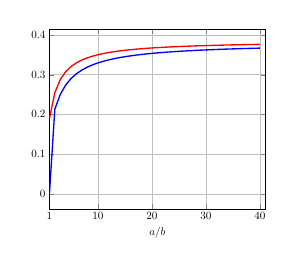
\begin{tikzpicture}[scale=0.4]
\begin{axis}[xlabel=$a/b$,ymajorgrids=true,xmajorgrids=true,xmin=1,xmax=41,xtick={1,10,20,30,40}]
%%%%%%%%%%% NATURAL CONFIGURATION
\addplot[Blue,very thick] coordinates {(1.0,-1.59364188514e-12) (2.0,0.212857320897) (3.0,0.249893924351) (4.0,0.27360416432) (5.0,0.290070593852) (6.0,0.30216822431) (7.0,0.311430129824) (8.0,0.318747857117) (9.0,0.324674954147) (10.0,0.329573175966) (11.0,0.333688883167) (12.0,0.337195633388) (13.0,0.340219213023) (14.0,0.342853009248) (15.0,0.345167807082) (16.0,0.347218235209) (17.0,0.349047125479) (18.0,0.350688533417) (19.0,0.352169876071) (20.0,0.3535134741) (21.0,0.354737683146) (22.0,0.355857736689) (23.0,0.356886382692) (24.0,0.357834370589) (25.0,0.358710828109) (26.0,0.359523555947) (27.0,0.360279260443) (28.0,0.360983738964) (29.0,0.361642028851) (30.0,0.362258527996) (31.0,0.362837093184) (32.0,0.36338112082) (33.0,0.363893613627) (34.0,0.364377236081) (35.0,0.364834360724) (36.0,0.365267107082) (37.0,0.365677374516) (38.0,0.36606687008) (39.0,0.366437132262) (40.0,0.366789551283) };
%%%%%%%%%%% MODIFIED CONFIGURATION
\addplot[Red,very thick] coordinates {(1.0,0.18887015067) (2.0,0.254459520239) (3.0,0.287403904864) (4.0,0.307169534548) (5.0,0.320334758075) (6.0,0.329729082668) (7.0,0.336768311765) (8.0,0.342238808871) (9.0,0.346612107914) (10.0,0.350188061313) (11.0,0.353166425063) (12.0,0.355685394958) (13.0,0.357843617559) (14.0,0.359713389803) (15.0,0.361348904135) (16.0,0.362791580609) (17.0,0.364073619671) (18.0,0.36522043174) (19.0,0.366252337065) (20.0,0.367185779335) (21.0,0.368034207917) (22.0,0.368808729666) (23.0,0.369518597597) (24.0,0.370171582133) (25.0,0.370774256583) (26.0,0.371332219112) (27.0,0.371850267081) (28.0,0.372332535292) (29.0,0.372782606539) (30.0,0.373203600747) (31.0,0.373598247379) (32.0,0.373968944663) (33.0,0.374317808349) (34.0,0.374646712123) (35.0,0.374957321245) (36.0,0.375251120754) (37.0,0.375529439201) (38.0,0.375793468735) (39.0,0.376044282167) (40.0,0.376282847537) };
\end{axis}
\end{tikzpicture}
%%% Local Variables:
%%% mode: latex
%%% TeX-master: "../../mainManuscript"
%%% End:
& \\ [2.75cm]
  %%%%%%%%%%%%%%%%%%%%%%%%%%%%%%%%%%%%%
  %%%%%%%%%%%%%%%%%%%%%%%%%%%%%%%%%%%%%
  \hline % Shifted above // Shifted below
  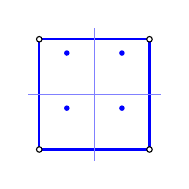
\begin{tikzpicture}[scale=0.7]
    \draw[Blue,thick] (-1.,-1.) rectangle (1.,1.);
    \draw[Blue!50] (-1.2,0.) -- (1.2,0.0);\draw[Blue!50] (.0,-1.2) -- (0.,1.2);
    %% nodes
    \fill[white] (-1,-1) circle (0.05);\draw (-1,-1) circle (0.05);
    \fill[white] (1.,-1) circle (0.05);\draw (1,-1) circle (0.05);
    \fill[white] (1,1) circle (0.05);\draw (1,1) circle (0.05);
    \fill[white] (-1.,1) circle (0.05);\draw (-1,1) circle (0.05);
    %% particles
    \fill[Blue] (-0.5,-0.5+0.25) circle (0.05);
    \fill[Blue] (0.5,-0.5+0.25) circle (0.05);
    \fill[Blue] (0.5,0.5+0.25) circle (0.05);
    \fill[Blue] (-0.5,0.5+0.25) circle (0.05);
  \end{tikzpicture} &  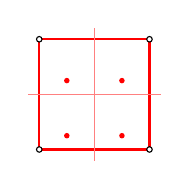
\begin{tikzpicture}[scale=0.7]
    \draw[Red,thick] (-1.,-1.) rectangle (1.,1.);
    \draw[Red!50] (-1.2,0.) -- (1.2,0.0);\draw[Red!50] (.0,-1.2) -- (0.,1.2);
    %% nodes
    \fill[white] (-1,-1) circle (0.05);\draw (-1,-1) circle (0.05);
    \fill[white] (1.,-1) circle (0.05);\draw (1,-1) circle (0.05);
    \fill[white] (1,1) circle (0.05);\draw (1,1) circle (0.05);
    \fill[white] (-1.,1) circle (0.05);\draw (-1,1) circle (0.05);
    %% particles
    \fill[Red] (-0.5,-0.5-0.25) circle (0.05);
    \fill[Red] (0.5,-0.5-0.25) circle (0.05);
    \fill[Red] (0.5,0.5-0.25) circle (0.05);
    \fill[Red] (-0.5,0.5-0.25) circle (0.05);
  \end{tikzpicture}& 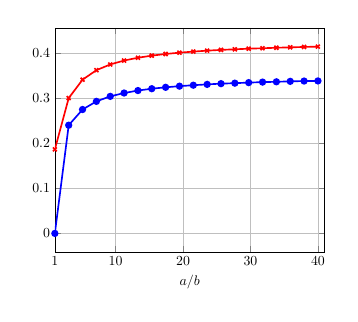
\begin{tikzpicture}[scale=0.5]
\begin{axis}[xlabel=$a/b$,ymajorgrids=true,xmajorgrids=true,xmin=1,xmax=41,xtick={1,10,20,30,40}]
%%%%%%%%%%% NATURAL CONFIGURATION
\addplot[Blue,mark=*,very thick] coordinates {(1.0,1.0000100001e-05) (3.05263157895,0.239878188256) (5.10526315789,0.274614851412) (7.15789473684,0.292689242682) (9.21052631579,0.303766195557) (11.2631578947,0.311204164673) (13.3157894737,0.316652640211) (15.3684210526,0.32074215479) (17.4210526316,0.323860607027) (19.4736842105,0.326382211191) (21.5263157895,0.328494863896) (23.5789473684,0.330344356075) (25.6315789474,0.331932266691) (27.6842105263,0.333044383075) (29.7368421053,0.334245447718) (31.7894736842,0.335382301191) (33.8421052632,0.336055465818) (35.8947368421,0.337054949497) (37.9473684211,0.337734956297) (40.0,0.338003380034) };
%%%%%%%%%%% MODIFIED CONFIGURATION
\addplot[Red,mark=x,very thick] coordinates {(1.0,0.186161861619) (3.05263157895,0.299954578493) (5.10526315789,0.340728670445) (7.15789473684,0.361763617636) (9.21052631579,0.374503745037) (11.2631578947,0.383176463344) (13.3157894737,0.389357577786) (15.3684210526,0.394050256292) (17.4210526316,0.397726608845) (19.4736842105,0.400577689987) (21.5263157895,0.402976661346) (23.5789473684,0.405090366693) (25.6315789474,0.406777225667) (27.6842105263,0.408069343851) (29.7368421053,0.409480410594) (31.7894736842,0.410406209325) (33.8421052632,0.411524115241) (35.8947368421,0.412434650662) (37.9473684211,0.413250974615) (40.0,0.414004140041) };
\end{axis}
\end{tikzpicture}
%%% Local Variables:
%%% mode: latex
%%% TeX-master: "../../mainManuscript"
%%% End:
 &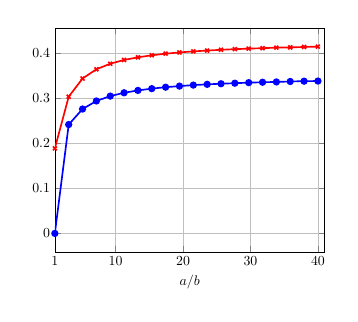
\begin{tikzpicture}[scale=0.5]
\begin{axis}[xlabel=$a/b$,ymajorgrids=true,xmajorgrids=true,xmin=1,xmax=41,xtick={1,10,20,30,40}]
%%%%%%%%%%% NATURAL CONFIGURATION
\addplot[Blue,mark=*,very thick] coordinates {(1.0,1.0000100001e-05) (3.05263157895,0.241770838761) (5.10526315789,0.276248551959) (7.15789473684,0.294120835945) (9.21052631579,0.304963575952) (11.2631578947,0.312330491726) (13.3157894737,0.317584754795) (15.3684210526,0.321510583527) (17.4210526316,0.324731668369) (19.4736842105,0.327161166349) (21.5263157895,0.329355925138) (23.5789473684,0.33105173157) (25.6315789474,0.332444903396) (27.6842105263,0.333598072823) (29.7368421053,0.334840190507) (31.7894736842,0.335700199107) (33.8421052632,0.336393890255) (35.8947368421,0.337413900455) (37.9473684211,0.338114433776) (40.0,0.338403384034) };
%%%%%%%%%%% MODIFIED CONFIGURATION
\addplot[Red,mark=x,very thick] coordinates {(1.0,0.188871888719) (3.05263157895,0.303648299641) (5.10526315789,0.343945018398) (7.15789473684,0.364483644836) (9.21052631579,0.376898505827) (11.2631578947,0.385203852039) (13.3157894737,0.391088647729) (15.3684210526,0.395587113766) (17.4210526316,0.399120306993) (19.4736842105,0.401940861514) (21.5263157895,0.404268253209) (23.5789473684,0.40603353402) (25.6315789474,0.407802499078) (27.6842105263,0.409176723346) (29.7368421053,0.410372524778) (31.7894736842,0.411359903073) (33.8421052632,0.412539388552) (35.8947368421,0.413152552578) (37.9473684211,0.414009929573) (40.0,0.414804148041) };
\end{axis}
\end{tikzpicture}
%%% Local Variables:
%%% mode: latex
%%% TeX-master: "../../mainManuscript"
%%% End:
& \\ [2.75cm]
  %\begin{minipage}{0.85\textwidth}\lipsum[1]\end{minipage}
\end{tabular}

%%% Local Variables: 
%%% mode: latex
%%% TeX-master: "../../mainManuscript"
%%% End: